%!TEX root = report.tex
\chapter{Data Collection and Generation}
\label{ch:data_generation}
\section{Overview}
\begin{figure}
\centering
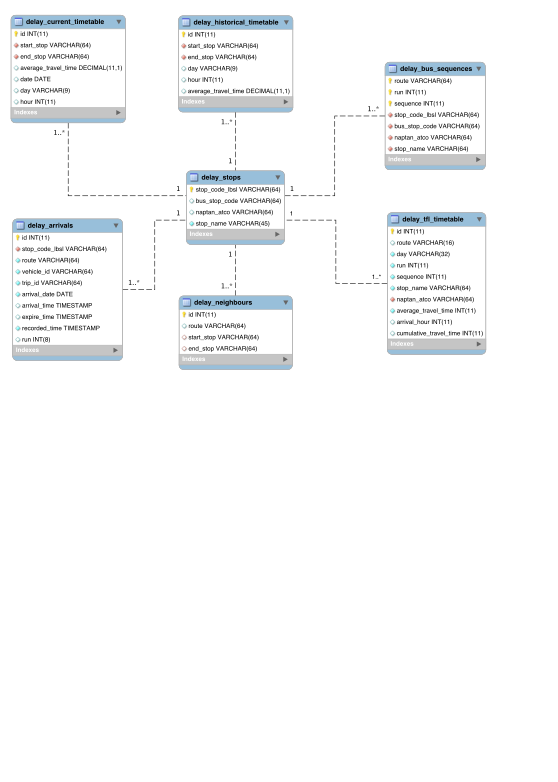
\includegraphics[width=\textwidth]{figures/uml.png}
\caption{\label{fig:uml} Databases Overview}
\end{figure}

\par This chapter discusses the backend development environment, and the detailed data collection and processing steps to generate the reference, current, and historical timetables. Figure \ref{fig:uml} shows the main tables in the Databases. We discussed the generation of these tables in the following sections.

\section{Development Environment}
\subsection{Virtual Machine}
\par We set up a Virtual Machine in the Doc's Private Cloud\cite{private_cloud} with the specifications shown in Table \ref{table:virtual_machine}. We allocated a large memory for memory intensive Databases operations.

\begin{table}
\centering
\begin{tabular}{@{}lr@{}} \toprule
Spec & Value \\ \midrule
Number of CPU Cores & 8 \\
CPU (in MHz) & 1000 \\
Memory (in GB) & 30 \\
 \bottomrule
\end{tabular}
\caption{Virtual Machine Specifications}
\label{table:virtual_machine}
\end{table}

\subsection{MySQL Databases}
\par We chose MySQL for backend data storage for the following reasons:

\begin{itemize}
  \item \textbf{User Interface} MySQL has convenient database management tools that enable easy data browsing, such as phpMyAdmin\cite{phpmyadmin} and Sequel Pro \cite{sequel_pro}.
  \item \textbf{Scalability} MySQL can handle memory-intensive computations efficiently once configured correctly.
\end{itemize}

\subsubsection{Databases Optimisation}
\par As some database operations involved joining large tables, we optimised the databases with the following settings in file \textit{/etc/mysql/my.cnf} to allow MySQL to access more memory in the Virtual Machine \cite{setting_innodb_buffer_pool_size,innodb_buffer}.

\begin{verbatim}
[mysqld]
innodb_io_capacity = 2000
innodb_read_io_threads = 64
innodb_thread_concurrency = 0
innodb_write_io_threads = 64
innodb_buffer_pool_size=20G
join_buffer_size=2G
sort_buffer_size=1G
read_buffer_size=1G
read_rnd_buffer_size=1G
max_connection=200
\end{verbatim}


